\section{Téléchargement des données}\label{sec:telechargement-des-donnes}

    \subsection{Généralité}\label{subsec:generalite}

    \begin{figure}[H]
        \begin{center}
            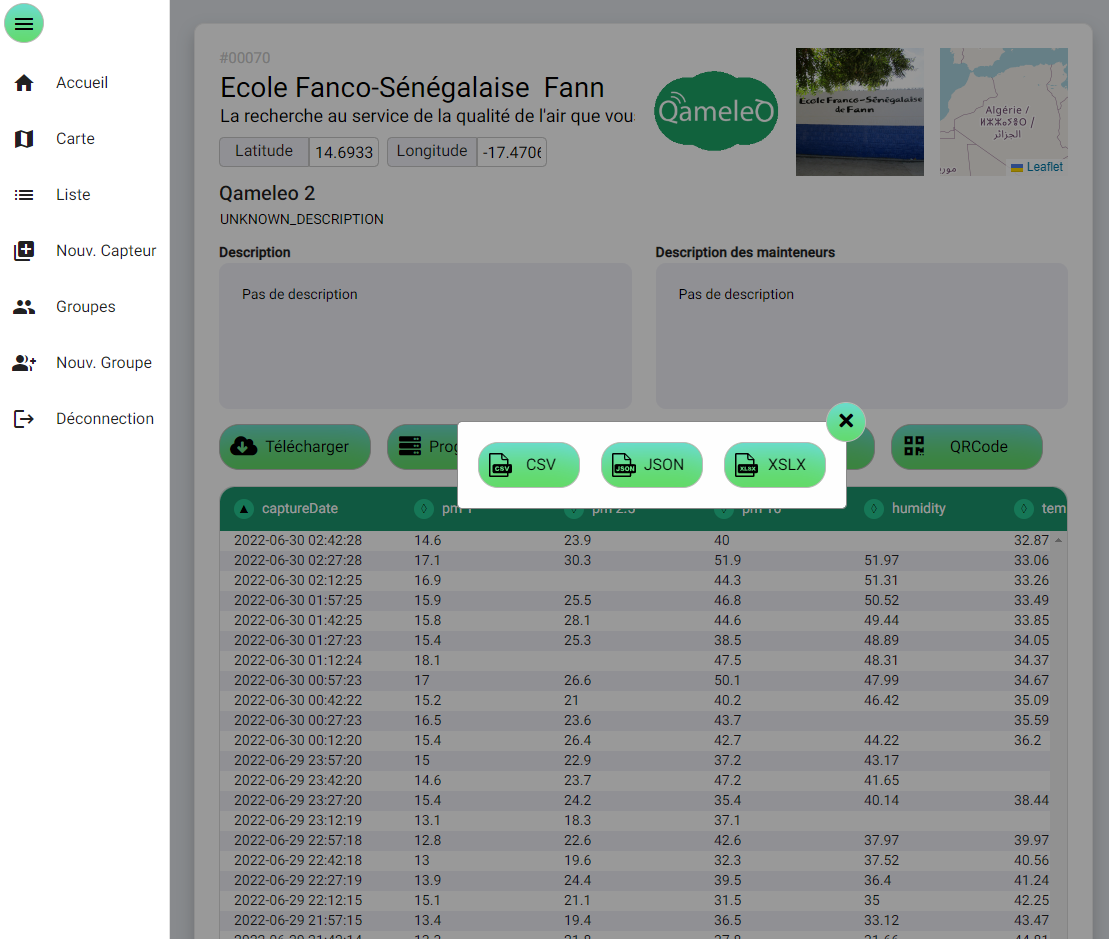
\includegraphics[width=12cm]{resources/sensor_download}
        \end{center}
        \caption{Téléchargement des données}\label{fig:telechargement-des-donnes}
    \end{figure}

    Après avoir appuyé sur ``Télécharger'' sur la page d'un capteur, une petite fenêtre
    s'ouvre vous demandant de choisir entre 3 formats, le format CSV, JSON et XSLX (Excel).
    Les formats CSV et JSON sont compressé via une archive ZIP pour permettre de les télécharger plus vite.

    \subsection{Format CSV}\label{subsec:csv}

    \begin{figure}[H]
        
\includegraphics[width=13cm]{resources/csv}
        \label{fig:csv}
    \end{figure}

    Le format csv possède 3 headers qu'il faudra ignorer : les noms, les identifiants, et les unités.
    Il faudra donc ignorer les 3 premières lignes.

    \begin{figure}[H]
        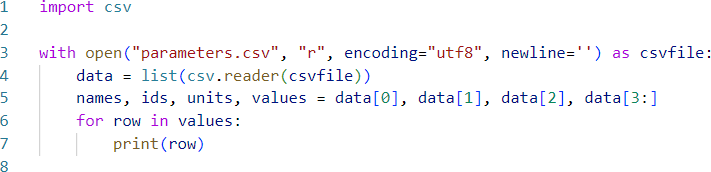
\includegraphics[width=11cm]{resources/csv_exemple}
        \caption{Script d'analyse de CSV}\label{fig:csv-exemple}
    \end{figure}

    Vous pouvez utiliser le script ci-dessus pour traiters les fichier CSV.

    \subsection{Format JSON}\label{subsec:json}

    \begin{figure}[H]
        
\includegraphics[width=13cm]{resources/json}
        \label{fig:json}
    \end{figure}

    Le format json est plus complet que le format CSV,  il contient en plus des informations sur le capteur et d'autres données.

    \begin{figure}[H]
        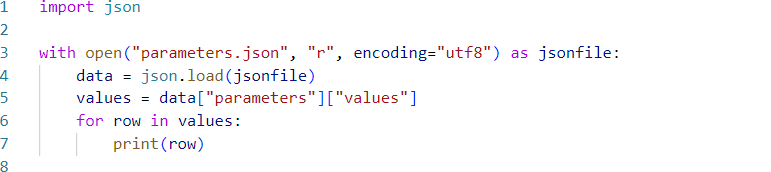
\includegraphics[width=11cm]{resources/json_exemple}
        \caption{Script d'analyse de JSON}\label{fig:json-exemple}
    \end{figure}

    Le script ci-dessus vous permettra le traitement des fichiers JSON.

    \subsection{Format XSLX}\label{subsec:xslx}

    \begin{figure}[H]
        \begin{center}
            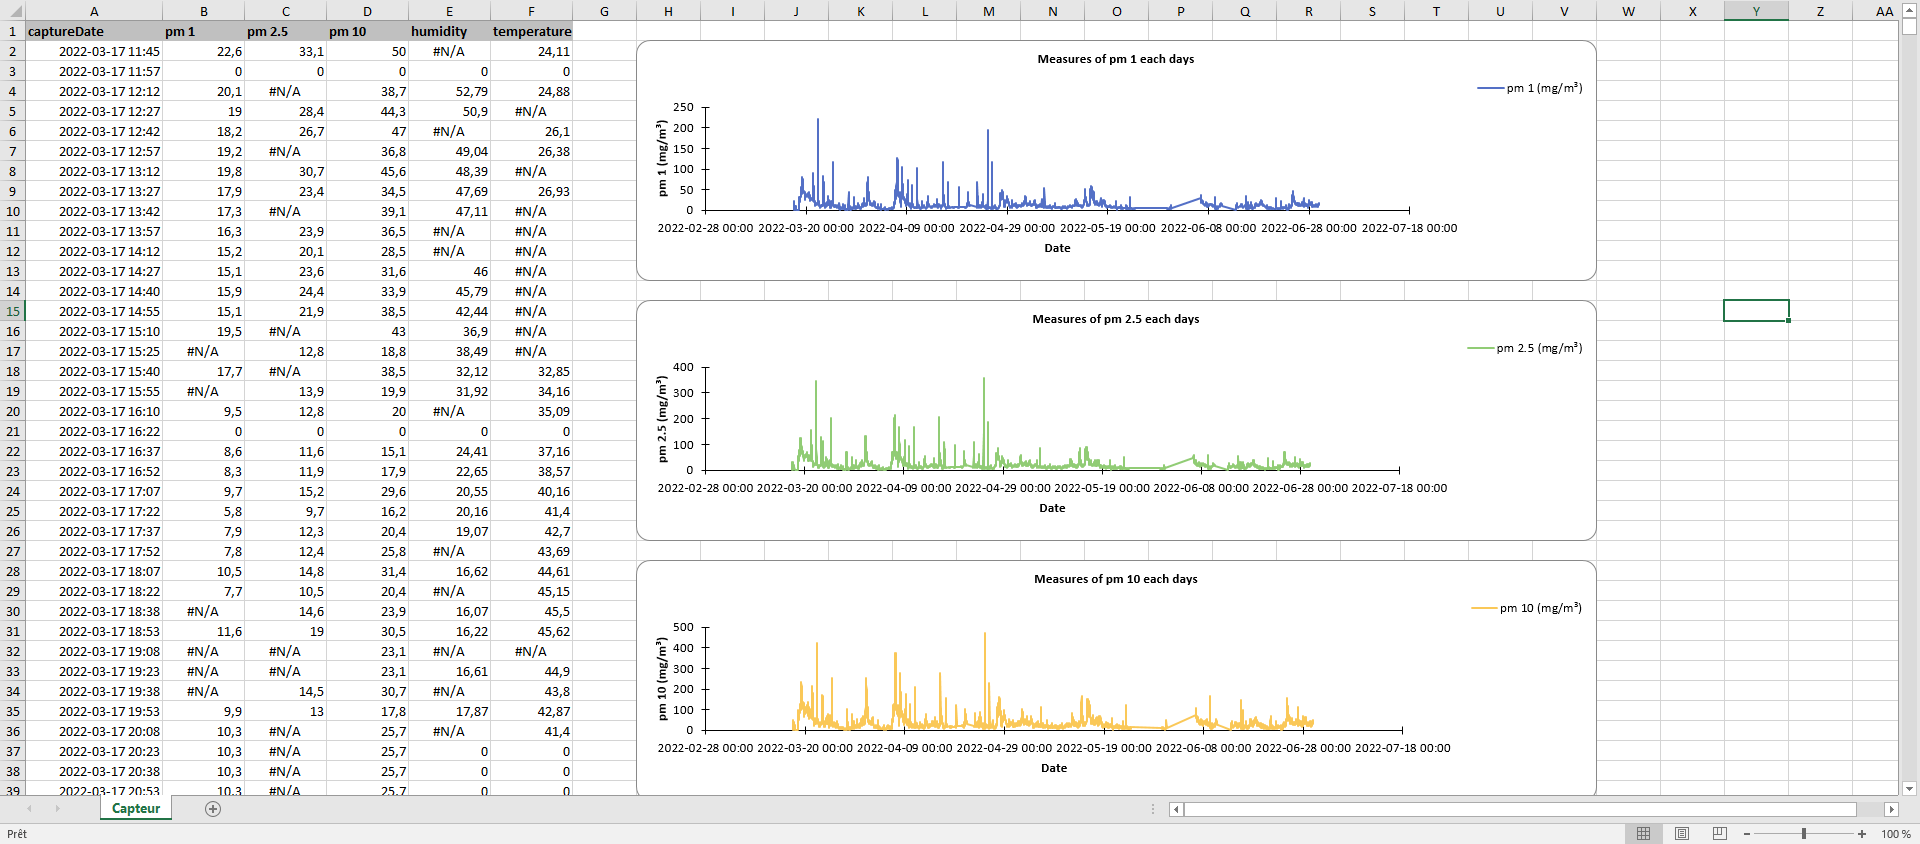
\includegraphics[width=14cm]{resources/xslx}
        \end{center}\label{fig:xslx}
    \end{figure}

    Le format XSLX est le format de fichier du logiciel Microsoft Excel.
    Vous aurez besoin de ce logiciel pour pouvoir ouvrir ce fichier.
    De plus, ce format comporte des courbes de données par défaut.

    \clearpage
